\documentclass{beamer}
\usetheme{Frankfurt}
\usetheme{CambridgeUS}
\usefonttheme{structuresmallcapsserif}
\usefonttheme{serif}
\setbeamertemplate{background canvas}[vertical shading][bottom=white,top=white]   
\setbeamercolor{math text}{fg=black!10!blue}
\setbeamercolor{block title}{bg=blue!40!white, fg=black}
\setbeamertemplate{navigation symbols}{}
\setbeamerfont{frametitle}{size=\normalsize}
\useoutertheme{mathASUlogo}
%\setbeamertemplate{enumerate items}[default]

\usepackage[utf8]{inputenc}
\usepackage[spanish]{babel}
\usepackage{amsmath}
\usepackage{amsfonts}
\usepackage{amssymb}
\usepackage{graphicx}
\usepackage{color}
\usepackage{listings}
\usepackage{hyperref}
\usepackage{wasysym}
\usepackage{alltt}
\usepackage{algorithmic}
\usepackage{cancel}
\usepackage{tikz}
\usetikzlibrary{arrows,backgrounds}
\tikzstyle{block}=[draw opacity=0.7,line width=1.4cm]

\graphicspath{{./Figuras/}{../Figuras/}{./}}
%\graphicspath{{./Figuras/}{../GGMC_2019/Figuras/}}

\definecolor{light-gray}{gray}{0.95}
\definecolor{light-blue}{rgb}{0.90,0.90,0.98}
\definecolor{light-yellow}{rgb}{0.95,0.95,0.10}
\definecolor{dark-green}{rgb}{0.10,0.50,0.10}

\definecolor{links}{rgb}{0.05,0.05,0.95}
\hypersetup{colorlinks,linkcolor=,urlcolor=links}

%%%%%%%%%%%%%%%%%%%%%%%%%%%%%% User specified LaTeX commands.
\newcommand{\Vector}[1]{{\underline{\mathbf{#1}}}}
\newcommand{\Tensor}[1]{{\underline{\underline{\mathbf{#1}}}}}
%%%%%%%%%%%%%%%%%%%%%%%%%%%%%%
% Definimos el punto decimal.
\spanishdecimal{.}
%%%%%%%%%%%%%%%%%%%%%%%%%%%%%%

%Global Background must be put in preamble
%\usebackgroundtemplate%
%{%
%$$\includegraphics[width=0.5\paperwidth]{python-logo}$$%
%}

% the beginning of each subsection:
\AtBeginSection[]
{
	\begin{frame}<beamer>{Contenido}
	\tableofcontents[currentsection]
\end{frame}
}

\title[GeoMaC]{Geof\'isica Matem\'atica y Computacional \\
%\textcolor{Lured}{\footnotesize{... }}\\
%\textcolor{Lured}{\footnotesize{...}}
}   
\author[\copyright LMCS, IGEF--UNAM]{Luis M. de la Cruz Salas} 
\institute[UNAM] 
{ 
{\small{Departamento de Recursos Naturales}} \\
\vspace{0.15cm}
{\small{Instituto de Geof\'isica}} \\ 
\vspace{0.15cm}
{\small{Universidad Nacional Aut\'onoma de M\'exico}} \\
\vspace{0.15cm}

\includegraphics[height=.85cm]{unamlogo.png} 
}

\date{\textcolor{Lured}{\footnotesize{Semestre 2021-I}}}

\subtitle{\textcolor{Lured}{Diferencias Finitas: Convección}}

% To uncover everything in a step-wise fashion:
%\beamerdefaultoverlayspecification{<+->}


\begin{document}

\begin{frame}
\titlepage
\end{frame}

\begin{frame}{Contenido}
\tableofcontents
\end{frame}

\section{Convección de calor}

\subsection{Modelo Conceptual}

\begin{frame}{}

{\huge MODELO}
$$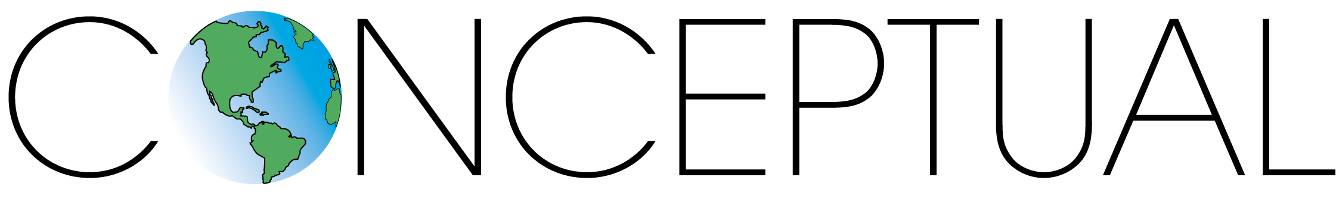
\includegraphics[height=1.5cm]{conceptualCOMPLETO}$$

\end{frame}

\begin{frame}{¿Qué es la convección de calor? \cite{Bergman}}
%
$$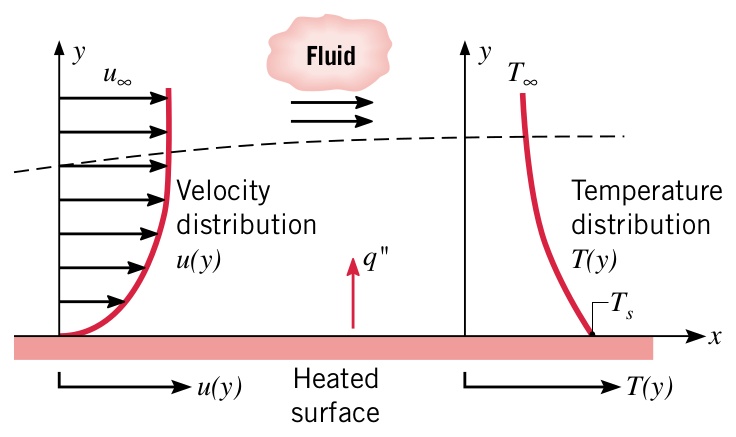
\includegraphics[scale=0.35]{conv01}$$
%
{\small La transferencia de calor por convección consiste de dos mecanismos:
\begin{itemize}
	\item \textbf{Difusión}: transferencia de energía debida al movimiento aleatorio molecular (difusión).
	\item \textbf{Advección}: movimiento de un fluido.
\end{itemize}
%
En la \textbf{convección}, el movimiento de un fluido en la presencia de un gradiente de temperaturas,
es lo que genera la transferencia de calor.}

\end{frame}


\begin{frame}{¿Qué es la convección de calor? \cite{Bergman}}
%
Transferencia de calor por convección.
%
$$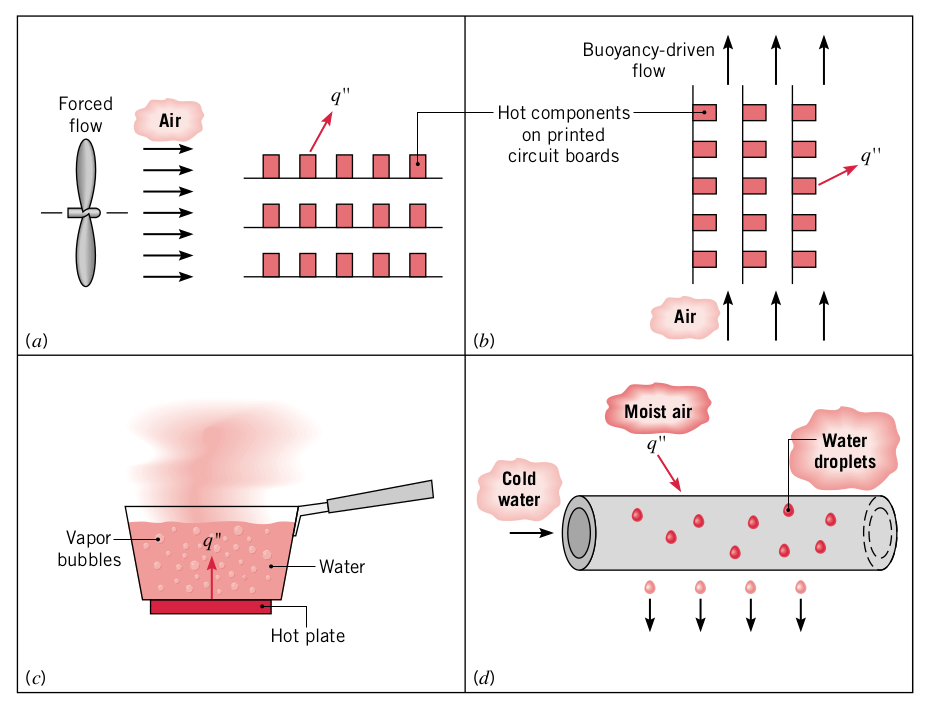
\includegraphics[scale=0.35]{conv02}$$
%
{\small (a) Forced convection. (b) Natural convection. (c) Boiling. (d) Condensation.}
\end{frame}


\subsection{Modelo Matemático}

\begin{frame}{}

{\huge MODELO}
$$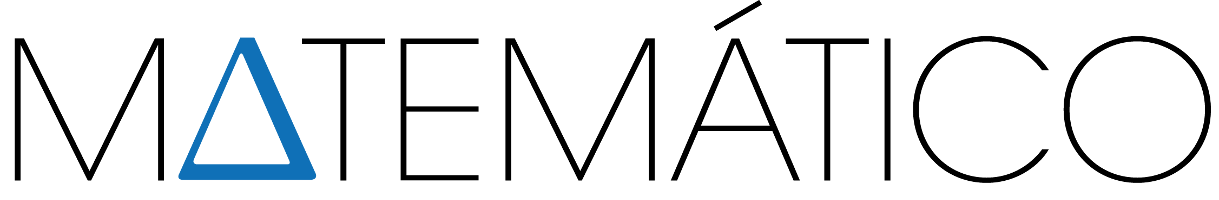
\includegraphics[height=1.5cm]{matematicoCOMPLETO}$$

\end{frame}


\begin{frame}{Ecuación "general" de transporte de calor}
%
\begin{equation}
c_p \rho \frac{\partial T}{\partial t} +
c_p \rho \frac{\partial}{\partial x_j} \left( u_j T \right) -
\frac{\partial }{\partial x_j} \left( \kappa \frac{\partial T}{\partial x_j}\right) = 
S
\end{equation}
%
{\footnotesize 
\begin{center}
	\begin{tabular}[h!]{cp{8cm}c}
		Símbolo &  & Unidades \\
		\hline
		\multicolumn{3}{c}{\textbf{Parámetros físicos}}\\
		$c_p$    & Capacidad calorífica específica. & [J / Kg $^\text{o}$K]\\
		$\rho$    & Densidad. & [Kg / m$^3$]\\
		$\kappa$ & Conductividad térmica. &  [W / m $^\text{o}$K] \\
		$S$ & Ganancia (fuente) o pérdida (sumidero) de calor & [J/m$^3$ s] \\
		
		$\displaystyle \alpha = \frac{\kappa}{c_p \rho}$ & Difusividad térmica. & [m$^2$/s] \\ \\
		\hline
		\multicolumn{3}{c}{\textbf{Variables independientes}}\\
		$x_j$    & Coordenadas de la posición: $(x_1, x_2, x_3) \equiv (x, y, z)$. & [m] \\
		$t$      & Tiempo. & [s] \\
		\hline
		\multicolumn{3}{c}{\textbf{Variables dependientes}}\\
		$T$    & Temperatura. & [$^\text{o}$K] \\
		$u_j$ & Componentes de la velocidad: $(u_1, u_2, u_3) \equiv (u_x, u_y, u_z)$. & [m/s] \\
		\hline
	\end{tabular}
\end{center}
}

\end{frame}

\begin{frame}{Casos especiales}

\begin{itemize}
	\item Conducción estacionaria
$$
-\frac{\partial }{\partial x_j} \left( \kappa \frac{\partial T}{\partial x_j}\right) = 
S
$$
	\item Conducción no estacionaria
$$
c_p \rho \frac{\partial T}{\partial t} -
\frac{\partial }{\partial x_j} \left( \kappa \frac{\partial T}{\partial x_j}\right) = 
S
$$
	\item Convección estacionaria
$$
c_p \rho \frac{\partial}{\partial x_j} \left( u_j T \right) -
\frac{\partial }{\partial x_j} \left( \kappa \frac{\partial T}{\partial x_j}\right) = 
S
$$
	\item Convección no estacionaria
$$
c_p \rho \frac{\partial T}{\partial t} +
c_p \rho \frac{\partial}{\partial x_j} \left( u_j T \right) -
\frac{\partial }{\partial x_j} \left( \kappa \frac{\partial T}{\partial x_j}\right) = 
S
$$
\end{itemize}
\end{frame}

\begin{frame}{Ejemplo 1: Convección estacionaria}

\begin{columns}
\begin{column}{0.5\textwidth}
{\footnotesize 
\begin{eqnarray*}
c_p \rho \frac{\partial}{\partial x} \left( u T \right) -
\frac{\partial }{\partial x} \left( \kappa \frac{\partial T}{\partial x}\right) & = &
S \\
T(0) & = & 1 \\
T(L) & = & 0
\end{eqnarray*}}
\end{column}
\begin{column}{0.5\textwidth}
$$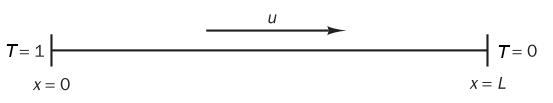
\includegraphics[scale=0.40]{conv03}$$
\end{column}	
\end{columns}


Usar $N = 6$ nodos igualmente espaciados y un esquema de diferencias finitas de segundo orden
para calcular la distribución de $T(x)$.

\begin{enumerate}
	\item $u = 0.1$ [m/s]
	\item $u = 2.5$ [m/s]
	\item $u = 2.5$ [m/s], con $N = 20$
\end{enumerate}

Datos: $L = 1.0$ [m], $\rho = 1.0$ [kg/m$^3$], $\kappa = 0.1$ [kg/m s], $S = 0$.

\end{frame}

\begin{frame}{Ejemplo 2: Convección NO estacionaria}

{\footnotesize 
\begin{eqnarray*}
	c_p \rho \frac{\partial T}{\partial t} +
	c_p \rho \frac{\partial}{\partial x_j} \left( u_j T \right) -
	\frac{\partial }{\partial x_j} \left( \kappa \frac{\partial T}{\partial x_j}\right) & = & S \\
	T(0, t) & = & 1 \qquad \text{para} \qquad 0 < t < t_{max} \\
	T(L, t) & = & 0 \qquad \text{para} \qquad 0 < t < r_{max} \\
	T(x, 0) & = & 0 \qquad \text{para} \qquad 0 < x \leq L
\end{eqnarray*}}

Usar un esquema de diferencias finitas de segundo orden para calcular la distribución de $T(x)$.
Encontrar un número de nodos $N$ para obtener una solución sin oscilaciones. 

\strut

Datos: $L = 2.5$ [m], $\rho = 1.0$ [kg/m$^3$], $u = 1.0$ [m/s], $\kappa = 0.001$ [kg/m s], $S = 0$, 
$h_t = 0.002$

\end{frame}

\subsection{Modelo Numérico}

\begin{frame}

{\huge MODELO}
$$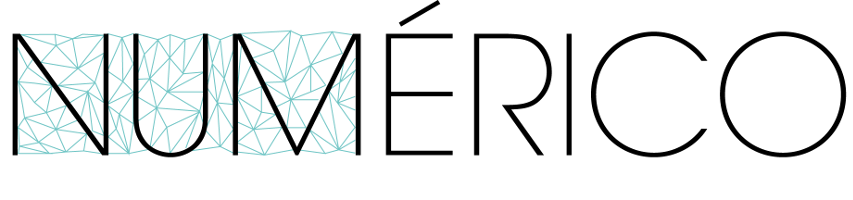
\includegraphics[height=1.75cm]{numericoCOMPLETO}$$

\end{frame}

\begin{frame}{Ejemplo 1: Convección estacionaria}
%
\[
\rho u \frac{d T}{d x} -
\kappa \frac{d^2 T}{d x^2} = S 
\]
%
$$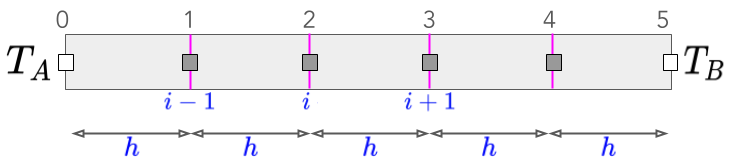
\includegraphics[height=1.5cm]{ModCon05}$$
%
{\small 
	\begin{eqnarray}
	\frac{d^2 T(x)}{dx^2} \Big|_i & \approx & \frac{T(x-h) - 2T(x) + T(x+h)}{h^2} = 
	\frac{T_{i-1} - 2T_{i} + T_{i+1}}{h^2} \nonumber \\
	\frac{d T(x)}{dx} \Big|_i & \approx & \frac{T(x+h) - T(x-h)}{2h} = \frac{T_{i+1} - T_{i-1}}{2h} \nonumber
	\end{eqnarray}
}
%
{\small 
	\[
	\rho u \left(\frac{T_{i+1} - T_{i-1}}{2h}\right) -
	\kappa \left(\frac{T_{i-1} - 2T_{i} + T_{i+1}}{h^2}\right) = S_i 
	\]
	
\begin{center}
	Para $i = 1 \dots N$.
\end{center}
}

\end{frame}

\begin{frame}{Ejemplo 1: Convección estacionaria}
%
\begin{center}
	Aproximación de orden $\mathcal{O}(h^2)$
\end{center}
%
\[
\boxed{
	-\left(\frac{\rho u}{2h} + \frac{\kappa}{h^2}\right) T_{i-1} +
	\frac{2\kappa}{h^2} T_i +
	\left(\frac{\rho u}{2h} - \frac{\kappa}{h^2}\right) T_{i+1} = S_i} \text{ para } i = 1 \dots N
\]
%
Sistema Lineal:
{\scriptsize 
	\[
	\left[
	\begin{array}{cccccc}
	\frac{2 \kappa}{h^2} & \frac{\rho u}{2 h} - \frac{\kappa}{h^2}   \\
	-\frac{\rho u}{2 h} - \frac{\kappa}{h^2} & \frac{2 \kappa}{h^2} & \frac{\rho u}{2 h} - \frac{\kappa}{h^2} \\
	\ddots & \ddots & \ddots &  \\
	&  -\frac{\rho u}{2 h} - \frac{\kappa}{h^2} & \frac{2 \kappa}{h^2} & \frac{\rho u}{2 h} - \frac{\kappa}{h^2}\\
	&  & -\frac{\rho u}{2 h} - \frac{\kappa}{h^2} & \frac{2 \kappa}{h^2} 
	\end{array}
	\right]
	\left[
	\begin{array}{c}
	T_1 \\ T_2 \\ \vdots \\ T_{N-1} \\ T_{N}
	\end{array}
	\right] =
	\left[
	\begin{array}{c}
	S_1 + \left(\frac{\rho u}{2 h} + \frac{\kappa}{h^2}\right)T_0 \\ 
	S_2 \\ 
	\vdots \\ 
	S_{N-1} \\ 
	S_{N} - \left(\frac{\rho u}{2 h} - \frac{\kappa}{h^2}\right)T_{N+1}
	\end{array}
	\right]
	\]
}

\strut
 
{\footnotesize Solución Analítica:
$\displaystyle
\boxed{
T(x) = \frac{\exp\left(\frac{\rho u x}{\kappa}\right) - 1 }{\exp\left(\frac{\rho v L}{\kappa}\right) - 1} (T_L - T_0) + T_0}
$}
\end{frame}


\begin{frame}{Ejercicio: Upwind}

Discretizar la ecuación  usando el esquema \textit{Upwind}:
%
\[
\rho u \frac{d T}{d x} -
\kappa \frac{d^2 T}{d x^2} = S 
\]
%
$$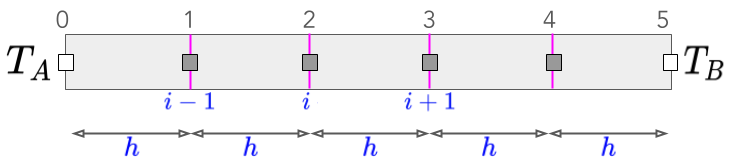
\includegraphics[height=1.5cm]{ModCon05}$$
%
%
{\footnotesize 
	\begin{eqnarray*}
	\frac{d^2 T(x)}{dx^2} \Big|_i & \approx & \frac{T(x-h) - 2T(x) + T(x+h)}{h^2} = 
	\frac{T_{i-1} - 2T_{i} + T_{i+1}}{h^2}  \\
	& & \boxed{\text{ Cuando } u > 0} \\
	\frac{d T(x)}{dx} \Big|_i & \approx & \frac{T(x) - T(x-h)}{h} = \frac{T_{i} - T_{i-1}}{h}  \\
	& & \boxed{\text{ Cuando } u < 0} \\
	\frac{d T(x)}{dx} \Big|_i & \approx & \frac{T(x+h) - T(x)}{h} = \frac{T_{i+1} - T_{i}}{h}  \\	
	\end{eqnarray*}
}


\end{frame}


\begin{frame}{Ejemplo 2: Convección NO estacionaria}
%
\[
\frac{\partial T}{\partial t} + 
u \frac{\partial T}{\partial x} -
\alpha \frac{\partial^2 T }{\partial x^2} = Q 
\]
%
$$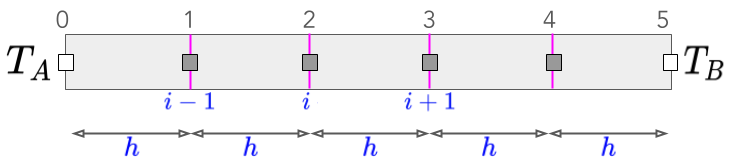
\includegraphics[height=1.5cm]{ModCon05}$$
%
{\small 
	\begin{eqnarray}
	\frac{\partial^2 T(x,t)}{dx^2} \Big|_i^n & \approx & \frac{T(x-h,t) - 2T(x,t) + T(x+h,t)}{h^2} = 
	\frac{T_{i-1}^n - 2T_{i}^n + T_{i+1}^n}{h^2} \nonumber \\
	\frac{\partial T(x,t)}{dx} \Big|_i^n & \approx & \frac{T(x+h,t) - T(x-h,t)}{2h} = \frac{T_{i+1}^n - T_{i-1}^n}{2h} \nonumber \\
	\frac{\partial T(x,t)}{\partial t} \Big|_i^n & \approx & \frac{T(x,t) - T(x,t-h_t)}{h_t} = \frac{T_i^{n} - T_i^{n-1}}{h_t} \nonumber
	\end{eqnarray}

\begin{center}
	Para $i = 1 \dots N$ y $n = 1 \dots N_t$.
\end{center}

}

\end{frame}

\begin{frame}{Ejemplo 2: Convección NO estacionaria}

{\small 
\[
\frac{T_i^n - T_i^{n-1}}{h_t} +
u \left(\frac{T_{i+1}^n - T_{i-1}^n}{2h}\right) -
\alpha \left(\frac{T_{i-1}^n - 2T_{i}^n + T_{i+1}^n}{h^2}\right) = Q_i 
\]
%
\begin{center}
	Aproximación de orden $\mathcal{O}(h^2, h_t)$
\end{center}
%
\[
\boxed{
	-\left(\frac{h_t u}{2h} + \frac{h_t \alpha}{h^2}\right) T_{i-1}^n +
	\left(\frac{2 h_t \alpha}{h^2} + 1\right) T_i^n +
	\left(\frac{h_t u}{2h} - \frac{h_t \alpha}{h^2}\right) T_{i+1}^n = Q_i + T_i^{n-1}}
\]

\begin{center}
	Para $i = 1 \dots N$ y $n = 1 \dots N_t$.
\end{center}

\strut

{\footnotesize Solución Analítica:
$\displaystyle
\boxed{
T(x,t) = 0.5  \left[\text{erfc}\left(\frac{x - ut}{2 \sqrt{\kappa t}}\right) +
					\exp\left(\frac{u x}{\kappa}\right)
					\text{erfc}\left(\frac{x + ut}{2 \sqrt{\kappa t}}\right) \right]
}
$
}

}

\end{frame}


\section{Advección pura}

\begin{frame}{Problema no estacionario: Advecci\'on pura}

Encontrar $u(x,t)$ que cumpla:
\[
\frac{\partial u}{\partial t} +  c \frac{\partial u}{\partial x}  = 0,
\,\,\, \text{ para } \,\,\, a \leq x \leq b, \,\,\, \text{ y } \,\,\, 0 \leq t \leq T_{max}.
\]

\begin{itemize}
\item Cond. inicial: $u(x,0) = \eta(x)$ ( + conds. de frontera $\Longrightarrow$ sol. \'unica).
\item Problema de Cauchy (PVI): 
\begin{itemize}
\item $-\infty \leq x \leq \infty$ 
\item Solo requiere de la condici\'on inicial.
\item El perfil inicial se mueve a velocidad $c$, es decir: $u(x,0) = \eta(x - c * t)$
\end{itemize}

\end{itemize}

\end{frame}

\begin{frame}{Esquemas de aproximaci\'on para Advecci\'on ($\left|\frac{c h_t}{h}\right| \leq 1$)}

\begin{itemize}
\item Orden de aprox. $\mathcal{O}(\Delta x^2 + \Delta t)$: 
\begin{displaymath}
u_{i}^{n+1} = u_{i}^{n} - \dfrac{c h_t}{2 h}\left(u_{i+1}^{n} - u_{i-1}^{n} \right)
\end{displaymath}	
\item \textit{Lax-Friedrichs Method} :
\begin{displaymath}
u_{i}^{n+1} =  \dfrac{1}{2}\left(u_{i-1}^{n} + u_{i+1}^{n}\right) - \dfrac{c h_t}{2 h}\left(u_{i+1}^{n} - u_{i-1}^{n} \right)
\end{displaymath}		
\item \textit{Leapfrog Method} :
\begin{displaymath}
u_{i}^{n+1} =  u_{i}^{n-1} - \dfrac{c h_t}{2 h}\left(u_{i+1}^{n} - u_{i-1}^{n} \right)
\end{displaymath}		
\item \textit{Lax-Wendroff Method} :
\begin{displaymath}
u_{i}^{n+1} = u_{i}^{n} - \dfrac{c h_t}{2 h}\left(u_{i+1}^{n} - u_{i-1}^{n} \right) + \dfrac{c^2 h_t^2}{2 h^2}\left(u_{i+1}^{n} - 2u_{i}^{n} + u_{i-1}^{n} \right)
\end{displaymath}	
({\footnotesize $u(x,t+\delta t) = u(x,t) + h_t u_t(x,t) + \frac{h_t^2}{2} u_{tt}(x,t)+\dots  $})

\end{itemize}

\end{frame}

\begin{frame}{Esquemas de aproximaci\'on para Advecci\'on }

\begin{itemize}
\item Upwind $c > 0$ (Estabilidad: $0 \leq \frac{c h_t}{h} \leq 1$): 
\begin{displaymath}
u_{i}^{n+1} = u_{i}^{n} - \dfrac{c h_t}{2 h}\left(u_{i}^{n} - u_{i-1}^{n} \right)
\end{displaymath}	
\item Upwind $c < 0$ (Estabilidad: $-1 \leq \frac{c h_t}{h} \leq 0$): 
\begin{displaymath}
u_{i}^{n+1} = u_{i}^{n} - \dfrac{c h_t}{2 h}\left(u_{i+1}^{n} - u_{i}^{n} \right)
\end{displaymath}
\item Beam-Warming $c > 0$ (Estabilidad: $0 \leq \frac{c h_t}{h} \leq 2$): 
\begin{displaymath}
u_{i}^{n+1} = u_{i}^{n} - \dfrac{c h_t}{2 h}\left(3u_{i}^{n} -4 u_{i-1}^{n} + u_{i-2}^n\right) + \dfrac{c^2 h_t^2}{2 h^2}\left(u_{i}^{n} - 2u_{i-1}^{n} + u_{i-2}^{n} \right)
\end{displaymath}	
\item Beam-Warming $c < 0$ (Estabilidad: $-2 \leq \frac{c h_t}{h} \leq 0$): 
\begin{displaymath}
u_{i}^{n+1} = u_{i}^{n} - \dfrac{c h_t}{2 h}\left(-3u_{i}^{n} +4 u_{i+1}^{n} - u_{i+2}^n\right) + \dfrac{c^2 h_t^2}{2 h^2}\left(u_{i}^{n} - 2u_{i+1}^{n} + u_{i+2}^{n} \right)
\end{displaymath}	

\end{itemize}

\end{frame}


\begin{frame}{Difusi\'on num\'erica }

{\small En el m\'etodo de Lax-Friedichs podemos escribir:
\begin{displaymath}
\dfrac{1}{2}\left(u_{i-1}^{n} + u_{i+1}^{n}\right) =  u_{i}^{n} + \dfrac{1}{2}\left(u_{i-1}^{n} - 2 u_{i}^{n} + u_{i+1}^{n}\right)
\end{displaymath}
Con lo que obtenemos:
\begin{displaymath}
u_{i}^{n+1} =  u_{i}^{n}  - \dfrac{c h_t}{2 h}\left(u_{i+1}^{n} - u_{i-1}^{n} \right) + \dfrac{1}{2}\left(u_{i-1}^{n} - 2 u_{i}^{n} + u_{i+1}^{n}\right)
\end{displaymath}		
Que se puede rearreglar como:
\begin{displaymath}
\left(\dfrac{u_{i}^{n+1} - u_{i}^{n}}{h_t}\right) + c\left(\dfrac{u_{i+1}^{n} - u_{i-1}^{n}}{2 h} \right) = \dfrac{h^2}{2h_t}\left(\dfrac{u_{i-1}^{n} - 2 u_{i}^{n} + u_{i+1}^{n}}{h^2}\right)
\end{displaymath}		
Esta \'ultima discretizaci\'on es similar a la obtenida de una ecuaci\'on como:
\begin{displaymath}
\dfrac{\partial u}{\partial t} + c \dfrac{\partial u}{\partial x} = \epsilon \dfrac{\partial^2 u}{\partial x^2}, \text{ para } \epsilon = h^2 / 2 h_t
\end{displaymath}
Para el m\'etodo de Upwind: $\epsilon = c h / 2$.

Para el m\'etodo de Lax-Wendroff: $\epsilon = c^2 h_t / 2$.
}

\end{frame}



\section<presentation>{Referencias}

\begin{frame}[allowframebreaks]
	%\frametitle<presentation>{Bibliograf\'{\i}a}
	
\begin{thebibliography}{10}
		
{\footnotesize 

% BOOKS 
\beamertemplatebookbibitems


\bibitem{Leveque}
[1] R.J. Leveque,
\newblock {\em Finite Difference Method for Ordinary and Partial Differential Equations: Steady State and Time-Dependent Problems },
\newblock {Society for Industrial and Applied Mathematics (SIAM), Philadelphia}, \textbf{2007}.

\bibitem{Saad}
[2] Y. Saad
\newblock {\em Iterative Methods for Sparse Linear Systems}.
\newblock PWS/ITP 1996.
\newblock {Online: 
	\textsf{http://www-users.cs.umn.edu/\textasciitilde saad/books.html}, 
	\textbf{2000}}

\bibitem{Burden}
[3]  Richard Burden and J. Douglas Faires
\newblock{\em Numerical Analysis}
\newblock Cengage Learning; 9 edition (August 9, \textbf{2010})

\bibitem{Herrera1} 
[4] I. Herrera \& G. F. Pinder,
\newblock {\em Mathematical Modeling in Science and Engineering: An Axiomatic Approach}, 
\newblock John Wiley \textbf{2012}.

% ARTICULOS    
\beamertemplatearticlebibitems

%\bibitem{Delacruz2011}
%[7]   L. M. de la Cruz,
%\newblock Flujo en una y dos fases en medios porosos: modelos matemáticos, numáricos y computacionales,
%\newblock {\em Reportes técnicos del Instituto de Geofísica}, 2012-4, Agosto \textbf{2012}.


}
		
\end{thebibliography}
\end{frame}

\end{document}
	